\documentclass[12pt,a4paper,oneside,brazil]{abntex2}
\usepackage[brazil]{babel}
\usepackage[utf8]{inputenc}
\usepackage[osf]{mathpazo}
\renewcommand{\familydefault}{\rmdefault}
\pagestyle{headings}
\setcounter{secnumdepth}{3}
\usepackage{lmodern}
\setcounter{tocdepth}{3}
\usepackage{amsmath, amsfonts, amssymb, amsthm, array}
\usepackage{float} 
\usepackage{calc, cases}
\usepackage[makeroom]{cancel}
\usepackage{nicefrac}

\usepackage{booktabs} 
\usepackage{subfig}
\usepackage{latexsym}
\usepackage[active]{srcltx}
\usepackage{graphicx} 
\graphicspath{ {figures/} }
\usepackage{indentfirst}
\usepackage{xcolor} 
\usepackage{url} 
\usepackage{relsize} 
\usepackage{microtype}
\OnehalfSpacing 
\makeatletter 
\pdfpageheight\paperheight 
\pdfpagewidth\paperwidth 
\providecommand{\tabularnewline}{\\} 
\raggedbottom 
\bookmarksetup{numbered} 
\setlength{\parindent}{1.3cm} 
\renewcommand{\cftsubsectionfont}{\footnotesize\normalfont\rmfamily} 
\renewcommand{\cftsectionfont}{\normalfont\rmfamily} 
\renewcommand{\ABNTEXchapterfont}{\rmfamily\fontseries{b}\selectfont} 
\usepackage{braket}
\usepackage{tikz}
\usepackage{tikz-3dplot}
\usetikzlibrary{hobby}
\usetikzlibrary{angles}
\usetikzlibrary{quotes}
\usepackage{eufrak}
\usepackage{epstopdf}
\usepackage[makeroom]{cancel}
\usepackage{physics}

%% Índices

\theoremstyle{definition}
\newtheorem{defin}{Definição}
\numberwithin{defin}{section}

\newtheorem{thm}{Teorema}
\numberwithin{thm}{section}

\newtheorem{notation}{Notação}
\numberwithin{notation}{section}

\theoremstyle{remark}

\newtheorem*{sol}{Solução}

\newtheorem{exmp}{Exemplo}
\numberwithin{exmp}{section}

\newtheorem*{obs}{Observação}
\newtheorem*{obss}{Observações}

\newtheorem*{prop}{Propriedade}
\newtheorem*{props}{Propriedade}

\newtheorem{p}{Proposição}
\numberwithin{p}{section}

\newtheorem{lema}{Lema}
\numberwithin{lema}{section}


%% Exemplos Especiais

\newtheorem*{exmp1}{Exemplo (Comutador)}


\newcommand\restr[2]{{
		\left.\kern-\nulldelimiterspace 
		#1 
		\vphantom{\big|} 
		\right|_{#2} 
}}

\newcommand{\xRightarrow}[2][]{\ext@arrow 0359\Rightarrowfill@{#1}{#2}}

\newcommand\numeq[1]%
{\stackrel{\scriptscriptstyle(\mkern-1.5mu#1\mkern-1.5mu)}{=}}

% Esse pacote pode ser editado. Por exemplo, onde está escrito {Autor}, dentro dos colchetes você pode colocar o seu nome, e assim por diante.

\hypersetup{
	pdftitle={Relatório de Iniciação Científica}, 
	pdfauthor={ARTHUR DE SOUZA MOLINA},
	pdfsubject={\imprimirpreambulo},
	pdfcreator={abnTeX2},
	pdfkeywords={Ferramentas para Explorar
		a Radiação Cósmica de Fundo e suas Anomalias}{Cosmologia}{Cálculo Numérico}{Estatística}{Correlação Cruzada},
	colorlinks=true,
	linkcolor=black, %Você pode mudar os cores dos links, i.e red, green, blue, etc.
	citecolor=black,
	filecolor=black,
	urlcolor=black,
	bookmarksdepth=4
}

\makeatother 



%% Novo estilo
\makepagestyle{estilo_pretextual} %%% escolha um nome
\makeevenhead{estilo_pretextual}{}{}{\ABNTEXfontereduzida \textbf \thepage}
\makeoddhead{estilo_pretextual}{}{}{\ABNTEXfontereduzida \textbf \thepage}

%% Customiza comando \pretextual
\renewcommand{\pretextual}{
	\pagenumbering{roman} %%% ou \pagenumbering{Roman}
	\aliaspagestyle{chapter}{estilo_pretextual}
	\pagestyle{estilo_pretextual}
	\aliaspagestyle{cleared}{empty}
	\aliaspagestyle{part}{estilo_pretextual}
}

\begin{document}

	\bookmarksetupnext{rellevel=-1}
	
	\pdfbookmark[1]{Capa}{Capa}
	\thispagestyle{empty}
	\begin{center}
		
\includegraphics[width=14.8cm]{figuras/logo} 
		\par\end{center}
	
	\begin{center}
		{\color{green!45!black} \rule{1\columnwidth}{1.5mm}}
		\par\end{center}
	
	\begin{center}
		\medskip{}
		\par\end{center}
	
	\begin{center}
		{\Large{}ARTHUR DE SOUZA MOLINA}
		\par\end{center}{\Large \par}
	
	\begin{center}
		\vfill{}
		\par\end{center}
	
	\begin{DoubleSpace}
		\begin{center}
			\textbf{\Large{}Ferramentas para Explorar
				a Radiação Cósmica de Fundo e suas Anomalias}
			\par\end{center}{\Large \par}
	\end{DoubleSpace}
	
	\begin{center}
		\vfill{}
		\par\end{center}
	
	\begin{center}
		{\color{green!45!black} \rule{1\columnwidth}{1.5mm}}
		\par\end{center}
	
	\begin{center}
		Londrina \\
		2021
		\par\end{center}
	
	\cleardoublepage{}
	
	\pdfbookmark[1]{Folha de rosto}{Folha de rosto}
	\thispagestyle{empty}
	\begin{center}
		{\Large{}ARTHUR DE SOUZA MOLINA}
		\par\end{center}{\Large \par}
	
	\begin{center}
		\vfill{}
		\par\end{center}
	
	\begin{DoubleSpace}
		\begin{center}
			\textbf{\Large{}Ferramentas para Explorar a Radiação Cósmica de Fundo e suas Anomalias}
			\par\end{center}{\Large \par}
	\end{DoubleSpace}
	
	\begin{center}
		\vfill{}
		
		\par\end{center}
	
	\noindent \begin{flushright}
		\begin{minipage}[c]{9.5cm}%
			Relatório de Iniciação Científica apresentado ao Departamento de Física da Universidade Estadual de Londrina, como requisito para o Programa de Iniciação Científica.
			
			Orientador: Prof. Dr. Sandro Dias Pinto Vitenti
		\end{minipage}
		\par\end{flushright}
	
	\vfill{}
	
	\begin{center}
		Londrina\\
		2021
		\par\end{center}
	
	\newpage{}
	
	\begin{folhadeaprovacao}
		\thispagestyle{empty}
		\begin{center}
			{\large{}ARTHUR DE SOUZA MOLINA}
			\par\end{center}{\large \par}
		
		\begin{center}
			\vfill{}
			\par\end{center}
		
		\begin{DoubleSpace}
			\begin{center}
				\textbf{\large{}Ferramentas para Explorar a Radiação Cósmica de Fundo e suas Anomalias}
				\par\end{center}{\large \par}
		\end{DoubleSpace}
		
		\begin{center}
			\vfill{}
			
			\par\end{center}
		
		\noindent \begin{flushright}
			\begin{minipage}[c]{9.5cm}%
				Relatório de Iniciação Científica apresentado ao Departamento de Física da Universidade Estadual de Londrina, como requisito para o Programa de Iniciação Científica.
				\begin{center}
					\vspace{1cm}
					\textbf{BANCA EXAMINADORA}
					\par\end{center}
				\vspace{1cm}
				
				\begin{SingleSpace}
					\begin{center}
						\underline{\hspace{9cm}}\\
						Orientador: Prof. Dr. Sandro Dias Pinto Vitenti \\
						Universidade Estadual de Londrina - UEL
						\par\end{center}
					\begin{center}
						\vspace{1cm}
						\underline{\hspace{9cm}}\\
						Prof. Dr. ...\\
						Universidade Estadual de Londrina - UEL
						\par\end{center}
					\begin{center}
						\vspace{1cm}
						\underline{\hspace{9cm}} \\
						Prof. Dr. ... \\
						Universidade Estadual de Londrina - UEL
						\par\end{center}
				\end{SingleSpace}
				\vspace{1cm}
				
				\begin{center}
					Londrina, \today %\_\_\_\_\_ de \_\_\_\_\_\_\_\_\_\_\_\_\_\_\_\_ de \_\_\_\_\_\_\_. 
					\par\end{center}%
			\end{minipage}
			\par\end{flushright}
		
	\end{folhadeaprovacao}
	\begin{agradecimentos}
		Agradeço a minha querida mãe pelo apoio incondicional, carinho, amor, estar comigo sempre e ser uma das pessoas mais importantes da minha vida.
		
		Agradeço ao meu orientador, Prof. Dr. Sandro Dias Pinto Vitenti por me conceder a oportunidade de produzir um projeto de iniciação cientifica, mesmo neste período de dificuldades que enfrentamos diariamente em virtude da pandemia de COVID-19.
		
		  
	\end{agradecimentos}
		
	\begin{SingleSpace}
		\noindent MOLINA, Arthur de Souza \textbf{Ferramentas para Explorar a Radiação Cósmica de Fundo e suas Anomalias}.
		2021. Relatório de Iniciação Científica para o Programa de Iniciação Científica \textendash{}
		Universidade Estadual de Londrina, Londrina, 2021.
	\end{SingleSpace}
	
	\setlength{\absparsep}{18pt}
	
	\begin{resumo}
		
		Com surgimento de diversos modelos cosmológicos, modificações no modelo padrão para explicar fenômenos ou novas teorias físicas e a evolução da tecnologia, tanto na questão da acessibilidade quanto na capacidade de processamento em computadores, surge a demanda por códigos de cosmologia que permitem fazer simulações, a previsão de resultados, verificar a coerência estatística em relação aos dados observacionais, cálculos mais otimizados para os conjuntos de dados que crescem exponencialmente com a produção de experimentos e o consenso dos resultados obtidos em cálculos numéricos entre os grupos de pesquisa. Neste trabalho, estudamos a descrição da formação de estruturas em grandes escala no universo com um tratamento Newtoniano através da instabilidade gravitacional e analisamos os códigos relacionados à correlações cruzadas das bibliotecas de cálculo numérico CCL e NumCosmo, afim de produzir um \textit{jupyter notebook} utilizando um algoritmo de validação do CCL como base para criar um teste de comparação dos cálculos numéricos feitos pelas bibliotecas utilizando o mesmo conjunto de dados, documentar a precisão entre as bibliotecas e os métodos com gráficos e verificar a concordância entre elas.
		
		\textbf{Palavras-chave:} Cosmologia. Cálculo Numérico.
		 Estatística. Correlações Cruzadas.
	\end{resumo}
	

	
	\begin{SingleSpace}
		\noindent Molina, Arthur de Souza \textbf{Tools for Exploring Cosmic Background Radiation and its Anomalies}. 2021.
		Scientific Initiation Report in Physics \textendash{} Universidade
		Estadual de Londrina, Londrina, 2021.
	\end{SingleSpace}
	
	\setlength{\absparsep}{18pt}
	
	\begin{resumo}[Abstract]
		
		\begin{otherlanguage*}{english}
			With the emergence of several cosmological models, modifications to the standard model to explain phenomena or new physical theories, and the evolution of technology, both in terms of accessibility and processing capacity in computers, there is a demand for cosmology codes that allow for simulations, the predicting results, verifying statistical coherence to observational data, more optimized calculations for datasets that grow exponentially with the production of experiments and the consensus of results obtained in numerical calculations among research groups. In this work, we study the description of the formation of large-scale structures in the universe with a Newtonian treatment through gravitational instability and analyze the codes related to cross-correlations from the CCL and NumCosmo numerical calculus libraries, to produce a \textit{jupyter notebook} using a CCL validation algorithm as a basis to create a test to compare the numerical calculations made by the libraries using the same dataset, document the accuracy between the libraries and the methods with graphs and verify the agreement between them. 
			
			\textbf{Keywords:} Cosmology. Numerical Calculation. Statistics. Cross-correlation.
		\end{otherlanguage*}
		
	\end{resumo}
	
	\pdfbookmark[0]{\listfigurename}{lof}
	
	\listoffigures*
	
	
	%\pdfbookmark[0]{\listtablename}{lot}
	
	%\listoftables*
	
	
	\cleardoublepage
	
	\pdfbookmark[0]{\contentsname}{toc}

	\tableofcontents*
	
	\cleardoublepage
	
	\textual
	\pagenumbering{arabic}
	\setcounter{page}{1}
	
		\chapter*{Introdução}
\addcontentsline{toc}{chapter}{Introdução}

 





		
		\chapter*{Instabilidade Gravitacional}
\addcontentsline{toc}{chapter}{Instabilidade Gravitacional}

Quando estudamos uma estrutura de grande escala utilizando as teorias Newtonianas, pressupomos que a estrutura não possui velocidade relativística, a estrutura está em uma região que se expande menos rapidamente em relação as outras regiões, a estrutura esteja em colapso sobre a sua auto-gravidade, ou seja, a instabilidade gravitacional é o mecanismo de maior contribuição para sua evolução e a matéria se comporta como um fluído perfeito.

A partir dessas pressuposições, podemos descrever essas estruturas em termos de sua distribuição de energia $\varepsilon(\mathbf{x},t)$, a entropia por unidade de massa $\textbf{S}(\mathbf{x},t)$ e o vetor velocidade $\textbf{V}(\mathbf{x},t)$, ao estabelecer essas quantidades para um volume fixo em uma região, sabemos que a variação da massa deve ser equivalente a variação de sua distribuição de energia em todo o volume nesta região, em outras palavras, 

\begin{equation}\label{eq1}
	\frac{dM}{dt} = \int_{\Delta V} \frac{\partial \varepsilon(\mathbf{x},t)}{\partial t} dV.
\end{equation}

A variação da massa também pode ser escrita como a variação do fluxo da distribuição de energia em todo o contorno do volume fixo

\begin{equation}\label{eq2}
	\frac{dM}{dt} = - \oint \varepsilon(\mathbf{x},t)\mathbf{V} d\sigma = - \int_{\Delta V} \nabla (\varepsilon(\mathbf{x},t)\mathbf{V}) dV.
\end{equation}

Devido a equivalência de eq. (1) e eq. (2), podemos escrever a seguinte relação consistente

\begin{equation}\label{eq3}
	\frac{\partial \varepsilon}{\partial t} + \nabla (\varepsilon\mathbf{V}) = 0,
\end{equation}

que nos permite lidar com a massa em termos de sua distribuição de energia e volume explicitamente. Podemos descrever instabilidade gravitacional na região, utilizando o conceitos como potencial gravitacional $\phi$, a segunda Lei de Newton e a pressão no fluído. A força gravitacional pode ser escrita como

\begin{equation}\label{eq4}
	\textbf{F}_{gr} = - \Delta M \nabla\phi,
\end{equation}

a força devido a pressão no fluído é dada por 

\begin{equation}\label{eq5}
	\textbf{F}_{pr} = - \oint p \cdot d\sigma = - \int_{\Delta V} \nabla p\,\,\, dV,
\end{equation}

ao utilizar a segunda Lei de Newton, podemos encontrar a equação de Euler

\begin{equation}\label{eq6}
	\dfrac{\partial \textbf{V}}{\partial t} + (\textbf{V} \cdot \nabla) \textbf{V} + \dfrac{\nabla p}{\varepsilon} + \nabla\phi = 0
\end{equation}

 que nos permite descrever a instabilidade gravitacional em termos do volume, distribuição de energia, a pressão e potencial gravitacional.
 
 A conservação de entropia do sistema não permite a dissipação de energia, e portanto, a entropia para um pequeno elemento de matéria é conservada
 
 \begin{equation}\label{eq7}
 	\dfrac{d S(\textbf{x},t)}{dt} = \dfrac{\partial S}{\partial t} + (\textbf{V} \cdot \nabla) S = 0,
 \end{equation} 
 
 também usamos a equação de Poisson para determinar o potencial gravitacional
 
 \begin{equation}\label{eq8}
 	\nabla^2\phi = 4\pi G\varepsilon.
 \end{equation}

Através dessas equações hidrodinâmicas, podemos estudar o comportamento de pequenas pertubações nas funções desconhecidas: $ \varepsilon $,$ \textbf{V} $, $ p $ e $ \phi $.

\section*{Teoria de Jeans}

Assumimos que o universo é estático, homogêneo, isotrópico, não expansível e que a distribuição de energia na região estudada não varia com tempo e permaneça constante $\varepsilon (\mathbf{x},t) = \text{constante}$, mas para que a distribuição de energia permaneça constante, a matéria necessitaria de estar em repouso, o fato da força gravitacional ser proporcional ao gradiente do potencial, não permite que essa condição seja satisfeita, ou seja, a equação de Poisson não é satisfeita, logo o universo precisar de uma constante de cosmológica apropriada para se manter estático.

Com pequenas pertubações, temos

\begin{equation}\label{eq9}
	\varepsilon (\textbf{x},t) = \varepsilon_0 + \delta\varepsilon (\textbf{x},t),\,\, \textbf{V} (\textbf{x},t) = \textbf{V}_0 +\delta\textbf{V} (\textbf{x},t) 
\end{equation}

$$\phi (\textbf{x},t) = \phi_0 + \delta\phi (\textbf{x},t), S (\textbf{x},t)= S_0 + \delta S (\textbf{x},t)$$

onde cada variação $\delta\varepsilon \ll \varepsilon_0$ e assim por diante. A pressão é dada por

\begin{equation}\label{eq10}
	p (\textbf{x},t) = p( \varepsilon_0 + \delta\varepsilon (\textbf{x},t), S_0 + \delta S (\textbf{x},t) ) = p_0 +\delta p (\textbf{x},t) 
\end{equation}

ao realizar uma aproximação linear dessas pertubações, podemos escrever a pertubação na pressão em termos da pertubação da distribuição de energia e a entropia assim

\begin{equation}\label{eq11}
	\delta p = c_s^2\delta\varepsilon + \sigma\delta S
\end{equation}

onde $c^2_s \equiv \left(\dfrac{\partial p}{\partial\varepsilon}\right)_s$ é o quadrado da velocidade do som e $\sigma \equiv \left(\dfrac{\partial p}{\partial S}\right)_\varepsilon$. Para a matéria não relativística, a velocidade do som é muito menor que a velocidade da luz ($c_s \ll c  $).

Através dessas pertubações nas variáveis do sistema, conseguimos construir uma descrição clara com aproximações lineares do comportamento do sistema. Ao aplicar as pequenas pertubações em cada uma das definições acima, combinando as equações, conseguimos obter uma relação de cada uma das variações ao mantendo apenas os termos lineares as pertubações da seguinte forma 

\begin{equation}\label{eq12}
	\dfrac{\partial^2\delta\varepsilon}{\partial t^2} - c^2_s\nabla^2\delta\varepsilon - 4\pi G\varepsilon_0\delta\varepsilon = \sigma\nabla^2\delta S(\textbf{x}),
\end{equation}

$ \delta\varepsilon $ está contida em uma equação fechada, onde a entropia serve como uma fonte da pertubação.

\subsection*{Pertubações adiabáticas}

No caso de uma pertubação adiabática, onde não há troca de calor, ou seja, a pertubação na entropia é nula, e portanto, não depende das coordenadas espaciais, uma vez que a entropia é o único termo da eq.(12) depende exclusivamente das coordenadas espaciais, consequentemente, o termo a direita da equação eq.(12) se torna equivalente a 0, logo ao utilizar as transformações de Fourier e encontrar uma equação diferencial que relaciona a pertubação da distribuição de energia com as quantidades expressas em uma equação completamente dependente do tempo dada por 

\begin{equation}\label{eq13}
	\dfrac{\partial^2 (\delta\varepsilon_k )}{\partial t^2} +(k^2c^2_s - 4\pi G\varepsilon_0)\delta\varepsilon_k (t) = 0
\end{equation}

a solução é dada por 

\begin{equation}\label{eq14}
	\delta\varepsilon_k (t) \propto e^{\pm \omega (t) i}
\end{equation}

onde $\omega (t) = \sqrt{k^2c^2_s - 4\pi G \varepsilon_0}$ e o comportamento da pertubação adiabática depende exclusivamente do sinal do expoente.

Definindo o comprimento Jeans como

\begin{equation}\label{eq15}
	\lambda_J = \dfrac{2\pi}{k_J} = c_S \left(\dfrac{\pi}{G\varepsilon_0} \right)^{1/2},
\end{equation}

onde $\omega (k_J) = 0$, para  $\lambda < \lambda_J$, as soluções descrevem as ondas sonoras, proporcionais a $ \delta\varepsilon_k \propto \sin (\omega t + \mathbf{k}\mathbf{x} + \alpha) $ que propaga com velocidade de fase 

\begin{equation}\label{eq16}
	c_{fase} = \dfrac{\omega}{k}= c_s\sqrt{1 - \dfrac{k^2_J}{k}}.
\end{equation}

Ao analisar as soluções, no limite de $k \geq k_J$ ou em escalas muito pequenas ($\lambda \leq \lambda_J$), onde a contribuição da gravidade é insignificante comparado com a contribuição da pressão, consequentemente $c_{fase} \to c_s$.\\

Uma dessas soluções descrevem o comportamento exponencialmente rápido e não homogêneo, enquanto outras correspondem o modo decaimento, onde $k \to 0$, $|\omega | t \to \dfrac{t}{t_{gr}}$, onde $t_{gr} \equiv (4\pi G\varepsilon_0)^{-1/2}$. Onde $t_{gr}$ é interpretado como o tempo característico de colapso para uma região com densidade de energia inicial $\varepsilon_0$.

O comprimento Jeans $\lambda_J \sim c_s t_{gr} $ é o "comunicação de som" sobre a qual a pressão consegue reagir as mudanças da densidade de energia devido ao colapso gravitacional.


\subsection*{Pertubações de Vetor}
No caso de uma pertubação de vetor, onde as pertubações na distribuição de energia e na entropia são nulas, ou seja, $ \delta\varepsilon = 0 $ e $ \delta S = 0$, ao aplicar este resultado nas equações hidrodinâmicas de pertubações e a transformação de Fourier, concluímos que a velocidade da pertubação de onda plana, isto é, $\delta\mathbf{v} = \mathbf{w_k} e^{i\mathbf{k}\mathbf{x}}$ e que a velocidade é perpendicular ao vetor de onda $\mathbf{k}$, ou seja,

\begin{equation}\label{eq17}
	\mathbf{w_k} \cdot \mathbf{k} = 0.
\end{equation}

 As perturbações vetoriais descrevem o movimento de cisalhamento do meio que não perturbam a densidade de energia, pois existem duas direções perpendiculares independentes para $\mathbf{k}$.
 
 \subsection*{Pertubações de Entropia}
 
 Por fim, as pertubações de entropia, onde $ \delta S \neq 0$, ao analisar a eq. (12) completa, aplicando as transformações de Fourier obtemos a seguinte equação diferencial 
 
\begin{equation}\label{eq18}
 	\dfrac{\partial^2 (\delta\varepsilon_k )}{\partial t^2} +(k^2c^2_s - 4\pi G\varepsilon_0)\delta\varepsilon_k  = -\sigma k^2 \delta S_k
\end{equation} 
 
 onde a solução geral é a combinação da solução da homogênea e da solução particular, para o caso independente do tempo $  \dfrac{\partial^2 (\delta\varepsilon_k )}{\partial t^2}  = 0 $, a solução é dada por 
 
\begin{equation}\label{eq19}
	\delta\varepsilon_k  = \dfrac{ -\sigma k^2 \delta S_k}{k^2c^2_s - 4\pi G\varepsilon_0}
\end{equation}

é chamada de pertubação de entropia. Observe-se que $k \to \infty$ quando a contribuição da gravidade não é relevante. Neste caso, a contribuição para a pressão devido à falta de homogeneidade da densidade de energia é exatamente compensada pela contribuição correspondente as perturbações de entropia, logo, essas pertubações ocorrem apenas em fluidos constituídos de muitas componentes, por exemplo, um fluido que consiste em bárions e radiação.

\section*{Universo em Expansão}

Ao considerarmos a instabilidade gravitacional no universo em expansão, homogêneo e isotrópico, onde a distribuição de energia depende do tempo e as velocidades obedecem a lei de Hubble-Lemaître, temos

\begin{equation}\label{eq20}
	\varepsilon = \varepsilon_0 (t), \,\,\, \mathbf{V} = \mathbf{V}_0 = \mathbf{H} (t) \mathbf{x}.
\end{equation}
 
 substituímos esse resultado na eq. (3), obtemos
 
\begin{equation}\label{eq21}
	\dfrac{\partial \varepsilon_0}{\partial t}  + 3 \mathbf{H}\varepsilon_0 = 0 
\end{equation} 

ao agruparmos a divergência equação de Euler com a equação de Poisson, chegamos na equação de Friedmann

\begin{equation}\label{eq22}
	\dot{\mathbf{H}} + \mathbf{H}^2 = - \dfrac{4\pi G}{3}\varepsilon_0,
\end{equation}

onde as pertubações são dadas por

\begin{equation}\label{eq23}
	\varepsilon = \varepsilon_0 + \delta\varepsilon_0 (\mathbf{x},t),\,\, \mathbf{V} = \mathbf{V}_0 + \delta\mathbf{v} , \phi= \phi_0 + \delta\phi\,\,\, 
\end{equation}

$$p = p_0 + \delta p= p_0 + c_2^2\delta\varepsilon ,$$

ao ignorar a pertubação de entropia. Podemos relacionar novamente as equações anteriores de hidrodinâmica com os termos lineares as pertubações e encontrarmos as equações hidrodinâmicas para um universo em expansão.

A velocidade de Hubble-Lemaître depende exclusivamente da posição $ \mathbf{x} $, portanto as transformações de Fourier não desacoplam as coordenadas eulerianas $ \mathbf{x} $ em equações diferenciais ordinárias dependentes exclusivamente do tempo. Logo, é mais conveniente utilizar as coordenadas Lagrangianas $ \mathbf{q} $ com  

\begin{equation}\label{eq24}
	\mathbf{x} = a(t)\mathbf{q},
\end{equation}

relacionando as operações diferenciais para uma função genérica 

\begin{equation}\label{eq25}
	\left(\dfrac{\partial}{\partial t}\right)_\mathbf{x} = \left( \dfrac{\partial}{\partial t} \right)_\mathbf{q} - (\mathbf{V}_0 \cdot \nabla_\mathbf{x}),
\end{equation}
 
as devidas espaciais estão relacionadas de forma mais simples

\begin{equation}\label{eq26}
	\nabla_\mathbf{x} = \dfrac{1}{a}\nabla_\mathbf{q},
\end{equation}

 introduzindo a amplitude fracionária de densidade de energia $ \delta \equiv \frac{\delta\varepsilon}{\varepsilon_0} $, podemos reescrever as equações hidrodinâmicas para um universo em expansão, a equação que descreve a conservação do fluxo de massa assume a forma 
 
 \begin{equation}\label{eq27}
 	\left( \dfrac{\partial \delta}{\partial t} \right) + \dfrac{1}{a}(\nabla\cdot\delta\mathbf{v}) = 0,
 \end{equation}
 
a equação de Euler é dada por

\begin{equation}\label{eq28}
	\left( \dfrac{\partial \delta\mathbf{v}}{\partial t} \right) +H\delta\mathbf{v}+\dfrac{c^2_s}{a}\nabla\delta + \dfrac{1}{a}\nabla\delta\phi =0
\end{equation}

e por fim, a equação de Poisson

\begin{equation}\label{eq29}
	\nabla^2\delta\phi = 4\pi Ga^2\varepsilon_0\delta
\end{equation}
 
e agrupando as equações relacionando seus resultados em termos lineares as pequenas pertubações, obtemos a equação que descreve a instabilidade gravitacional no universo em expansão que dado por
 
\begin{equation}\label{eq30}
 	\ddot{\delta} + 2\mathbf{H}\dot{\delta} - \dfrac{c^2_s}{a^2}\nabla^2\delta - 4\pi G\varepsilon_0\delta = 0.
\end{equation}

\subsection*{Pertubações adiabáticas}

No caso de pertubações adiabáticas no universo em expansão, utilizando a descrição da amplitude fracionária de densidade de energia no espaço de Fourier, obtemos a seguinte equação diferencial 

\begin{equation}\label{eq31}
	\ddot{\delta_\mathbf{k}} + 2\mathbf{H}\dot{\delta_\mathbf{k}} + \left( \dfrac{c^2_s k^2}{a^2} -4\pi G\varepsilon_0\right)\delta_\mathbf{k} = 0,
\end{equation} 

onde o comportamento de cada pertubação depende especialmente do tamanho espacial e o comprimento de Jeans é dado por

\begin{equation}\label{eq32}
	\lambda^{ph}_J = \dfrac{2\pi a }{k_J} = c_s\sqrt{\dfrac{\pi}{G\varepsilon_0}}
\end{equation}

onde $\lambda^{ph}$ é o comprimento de onda físico, relacionando
ao comprimento de onda comovente $\lambda = \dfrac{2\pi}{k}$ com $\lambda^{ph} = a\lambda$. Em um universo plano dominado pela matéria $\varepsilon_0 = (6\pi G t^2)^{-1}$ e, portanto,

\begin{equation}\label{eq33}
	\lambda_J^{ph} \sim c_s t,
\end{equation}

isto é, o comprimento do Jeans está na ordem do horizonte de som. Às vezes, ao  invés de usar o comprimento de Jeans, usa-se a massa de Jeans, definida como $M_J \equiv\varepsilon_0 (\lambda_J^{ph})^3$. Se $ c_s $ mudar diabaticamente, a solução particular da eq. (31) é dada por

\begin{equation}\label{eq34}
	\delta_\mathbf{k} \propto \dfrac{1}{\sqrt{c_s a}} \,exp\left( \pm k \int \dfrac{c_s dt}{a}\right)
\end{equation}

Em escalas muito maiores do que a escala de Jeans, a gravidade possui a maior contribuição na evolução da pertubação domina e negligencia o termo dependente de k em eq.(31). Então, uma das soluções é simplesmente e proporcional a constante de Hubble. Entretanto, ao substituir essa solução  $\delta_d = H (t)$ na eq.(31) e assumindo $c^2_s k^2 = 0$, descobre-se que a equação resultante coincide com o tempo derivada da equação de Friedmann eq.(22). Observe que $\delta_d = H (t)$ é o decaimento
solução da equação de perturbação ($ H $ diminui com o tempo) em um dominado pela matéria universo com curvatura arbitrária.

Quando utilizamos as propriedades da derivada do Wronskiano para encontrar soluções descobrimos que as soluções são proporcionais termos lineares a potência do tempo, portanto, vemos que em um universo em expansão, a instabilidade gravitacional é muito menor eficiente e a amplitude da perturbação aumenta apenas com a potência do tempo.

\subsection*{Pertubações de vetor}

No caso de pertubações de vetor em um universo em expansão, ou seja, substituindo $ \delta = 0$ nas equações hidrodinâmicas, obtemos

\begin{equation}\label{eq35}
	\nabla\delta\mathbf{v} = 0 , \quad \dfrac{\partial\delta\mathbf{v}}{\partial t } + H\delta\mathbf{v} = 0
\end{equation}

A primeira equação segue que para uma perturbação de onda plana, $\delta\mathbf{v} \propto \delta\mathbf{v}_\mathbf{k} (t)e^{(i\mathbf{kq})}$ e a velocidade peculiar $\delta\mathbf{v}$ é perpendicular ao número de onda $\mathbf{k}$. A segunda equação torna-se

\begin{equation}\label{eq36}
	\delta\dot{\mathbf{v}}_\mathbf{k}+ \dfrac{\dot{a}}{a}\delta\mathbf{v}_\mathbf{k}=0,
\end{equation}

e tem a solução $\delta\mathbf{v_k} \propto \frac{1}{a}$. Assim, as perturbações do vetor decaem conforme o
o universo se expande e podem ter amplitudes significativas no presente
apenas se suas amplitudes iniciais fossem tão grandes que estragassem completamente a isotropia do universo primordial. Em um universo inflacionário, não há espaço para grandes perturbações vetoriais primordiais e não desempenham qualquer papel na formação de
a estrutura em grande escala no universo. Perturbações de vetor, no entanto, podem ser
gerado tardiamente, após a estrutura não linear ter sido formada e pode explicar a rotação das galáxias por exemplo.
		\chapter*{Análise dos códigos}
\addcontentsline{toc}{chapter}{Análise dos códigos}

\subsection*{O algoritmo de validação}

Para realizar a comparação entre as observáveis, utilizamos como base um dos algoritmos do conjunto de teste de validação do CCL, o algoritmo de verificação dos cálculos de correlações cruzadas escrito em python chamado  \textit{test\_correlation.py}.

Este algoritmo consulta um conjunto de dados de redshift, o espectro de potência angular, contraste de densidade de matéria, multipolos correspondentes ao espectro de potência de entrada, spin e entre outras grandezas cosmológicas para inicializar os traçadores, ou seja, as funções de correlação. Ele calcula o valor da função de correlação para as separações angulares fornecidas como entrada e verifica a coerência do resultado comparando com o valor do erro de cálculo estimulado.

O algoritmo utiliza a estrutura de testes escalonáveis do módulo \textit{pytest} para validar os cálculos em 112 testes utilizando três traçadores:  \textit{NumberCountsTracer}, \textit{WeakLensingTracer} e \textit{CMBLensingTracer}. Os testes foram feitos com os métodos: \textit{fftlog} (Transformações rápidas de Fourier que permite menos custo computacional de processamento do que computar integrações de força bruta nos cálculos) e \textit{bessel} (método de cálculo utilizando as funções esféricas de Bessel), mas o método \textit{legendre} (Soma da força bruta sobre os polinômios de Legendre) não foi implementado.

O algoritmo consulta 35 arquivos com extensão \textit{.txt} contendo o conjunto de dados, mas apenas quatro arquivos são utilizados para realizar os cálculos dos observáveis e 31 arquivos são consultados para calcular o erro estimado e validar cada um dos cálculos realizados. O algoritmo possui um problema relativamente simples de implementação relacionado a declaração do endereço do diretório dos arquivos, onde é preciso realizar uma alteração no código para que o teste de validação funcione corretamente. 

\subsection*{A produção do jupyter notebook}
Um dos interesses deste trabalho era utilizar os testes com o traçador \textit{CMBLensingTracer}, ou observáveis com spin-0 utilizando outros traçadores, afim de comparar os resultados do teste com os resultados computados pela NumCosmo utilizando os mesmos conjuntos de dados e verificar o grau de concordância entre as bibliotecas sobre esses resultados, mas infelizmente, nenhum teste com essas condições foi implementado neste algoritmo. A NumCosmo ainda não possui suporte para observáveis com spin diferente de zero e, portanto, dentre os testes do algoritmo de validação, apenas os testes utilizando o traçador  \textit{NumberCountsTracer} com spin-0 permitem a continuidade do trabalho. O algoritmo possui suporte para computar tanto os casos analíticos quanto os casos de histograma, como os cálculos de casos analíticos não foram implementados na NumCosmo, este trabalho aborda apenas casos com  os dados de histograma para a comparação entre bibliotecas, mas este fato não impede de realizarmos a comparação dos métodos diferentes em casos analíticos feitos pelo CCL.

Ao adaptar o teste que utiliza o traçador \textit{NumberCountsTracer} e observáveis com spin-0 em um \textit{jupyter notebook} descartando a dependência da consulta dos 31 arquivos de validação dos resultados, a inicialização de outros traçadores e seus respectivos cálculos e assim, surgem dois desafios sobre a estrutura do código para a implementação, que seria remover a dependência do módulo \textit{pytest} e da consulta do conjunto de dados. A estrutura de testes escalonáveis do módulo \textit{pytest} é incompatível com o tipo de análise que precisamos e a consulta em vários arquivos não é interessante, pois o conjunto de dados é relativamente pequeno e podemos evitar as complicações, em outras palavras, buscamos a produção de um algoritmo simples sem complicações/problemas a mais para lidar.

Com auxílio de algoritmos simples escritos em python, aproveitamos a versatilidade da linguagem para extrair os dados dos arquivos consultados e agrupamos em uma coleção ordenada dos dados nas listas dentro do \textit{jupyter notebook}. Em um estudo detalhado do comportamento do algoritmo e suas diversas funções escalonadas no teste e várias tentativas de sintetizar o código, foi possível simplificar todas as funções do algoritmo em apenas uma função, com poucas entradas, eliminando as verificações de envio de parâmetro inválidos e com os mesmos resultados que o algoritmo original apresentava.

Reaproveitamos uma função de comparação de resultados entre o CCL e a NumCosmo para a produção dos gráficos de distâncias relativas, ela é responsável por construir dois gráfico organizados na horizontal, onde o primeiro apresentava as curvas dos resultados de ambas as bibliotecas e o segundo, a curva da distância relativa dos seus cálculos. A função estava definida no \textit{jupyter notebook} presente no repositório da NumCosmo chamado \textit{NumCosmoCCLTest.ipynb}, onde apresentava a comparação dos resultados computados de distância e espectro de potência de ambas as bibliotecas, demostrando a discordância/concordância de seus cálculos.

Após o tratamento do algoritmo com os dados computados pelo CCL, desenvolvemos um estudo sobre a implementação dos códigos da NumCosmo ao estudar, documentar e separar os códigos anteriores do arquivo \textit{NumCosmoCCLTest.ipynb} em três arquivos que realizam a comparação dos resultados de distância, espectro de potência e o que produzimos sobre correlações cruzadas entre as bibliotecas com o objetivo de aprender a introspecção da NumCosmo no \textit{python}.











		\chapter*{Resultados}
\addcontentsline{toc}{chapter}{Resultados}

Através da função de construção de gráficos mencionado anteriormente, foi possível construir diversos gráficos para a comparação de métodos, funções de correlação e os resultados entre as bibliotecas usando o traçador \textit{NumberCountTracer}. 

\subsection*{Comparação dos cálculos do CCL usando os dados do caso de histograma}

Ao comparar os cálculos realizados com mesma função de correlação usando os métodos \textit{fftlog} e \textit{bessel}, os dados do caso de histograma obtemos os seguintes gráficos.

\begin{figure}[h!]
	\centering
	\caption{Comparação entre os métodos \textit{fftlog} e o \textit{bessel} para a mesma função de correlação no caso de histograma.}
	\label{fig:fig1}
	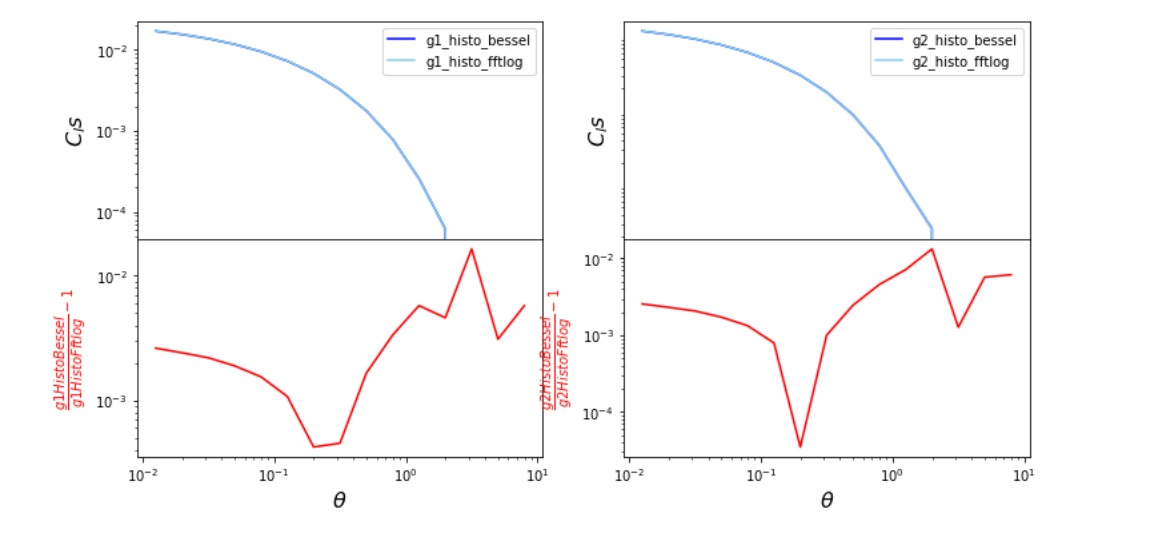
\includegraphics[width=0.7\linewidth]{figuras/fig1}
	
	Fonte: O jupyter notebook \textit{NumCosmoCCLTest\_Cross-Correlation.ipynb}.
\end{figure}

As curvas plotadas nos primeiros gráficos mostram que os cálculos convergem e a distância relativa entre os valores calculados utilizando métodos diferentes concordam entre si com uma precisão média de $ 10^{-3} $ entre os valores calculados. 

\newpage
Em seguida, ao comparar as curvas dos cálculos com funções de correlação diferentes com o mesmo método e os dados de histograma obtemos o seguinte gráfico:

\begin{figure}[H]
	\centering
	\caption{Comparação os mesmos métodos e diferentes funções de correlação no caso de histograma.}
	\label{fig:fig2}
	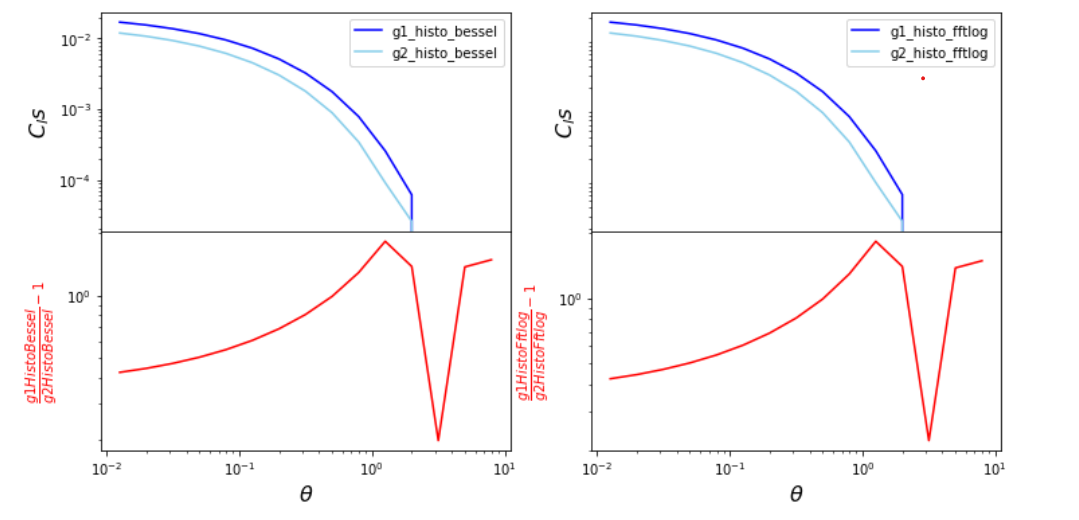
\includegraphics[width=0.7\linewidth]{figuras/fig2}
	
	Fonte: O jupyter notebook \textit{NumCosmoCCLTest\_Cross-Correlation.ipynb}.
\end{figure}

As curvas dos cálculos plotados nos primeiros gráficos não convergem para os mesmos pontos, porém possuem o mesmo comportamento. A distância relativa entre os valores calculados utilizando os mesmos métodos em diferentes funções de correlação possuem pouca concordância entre si com uma precisão média de $ 10^0 $.

\subsection*{Comparação dos cálculos do CCL usando os dados do caso analítico}

Ao comparar os cálculos realizados com mesma função de correlação usando os métodos \textit{fftlog} e \textit{bessel}, os dados do caso analítico, obtemos os seguintes gráficos. 

\begin{figure}[H]
	\centering
	\caption{Comparação entre os métodos \textit{fftlog} e o \textit{bessel} utilizando os dados do caso analíticos.}
	\label{fig:fig3}
	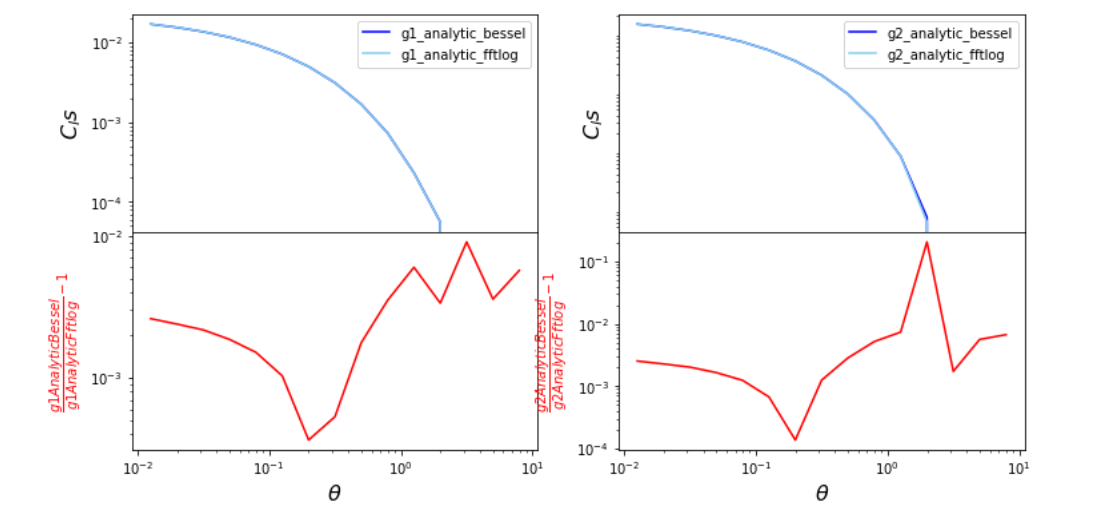
\includegraphics[width=0.7\linewidth]{figuras/fig3}
	
	Fonte: O jupyter notebook \textit{NumCosmoCCLTest\_Cross-Correlation.ipynb}.
\end{figure}

As curvas plotadas nos primeiros gráficos mostram que os cálculos convergem e a distância relativa entre os valores calculados utilizando métodos diferentes concordam entre si com uma precisão média de $ 10^{-3} $ entre os valores calculados. Por fim, comparamos os mesmos métodos para diferentes funções de correlação e obtemos os seguintes gráficos:

\begin{figure}[H]
	\centering
	\caption{Comparação dos mesmos métodos para calcular funções de correlação diferentes utilizando os dados do caso analítico.}
	\includegraphics[width=0.7\linewidth]{"figuras/fig4"}
	
	\label{fig:fig4}
	
	Fonte: O jupyter notebook \textit{NumCosmoCCLTest\_Cross-Correlation.ipynb}.
\end{figure}

A distância relativa na quarta análise demostra que os resultados apresentam pouca precisão e pouca concordância entre si, mas segue um comportamento semelhante.

\subsection*{Comparação entre os resultados do CCL e da NumCosmo}

Para a comparação entre os cálculos da NumCosmo e do CCL, usamos os resultados calculados pela NumCosmo com o método \textit{CVODE} e o conjunto de dados do caso de histograma, comparando uma função de correlação por vez, usando o mesmo método e função de correlação por ambas as bibliotecas e assim obtemos os seguintes gráficos: 

\begin{figure}[H]
	\centering
	\caption{Comparação dos cálculos usando o método \textit{bessel} e a função de correlação g1 por ambas as bibliotecas.}
	\includegraphics[width=0.7\linewidth]{"figuras/fig5"}	
	\label{fig:fig5}
	
	Fonte: O jupyter notebook \textit{NumCosmoCCLTest\_Cross-Correlation.ipynb}.
\end{figure}

\begin{figure}[H]
	\centering
	\caption{Comparação dos cálculos usando o método \textit{fftlog} e a função de correlação g1 por ambas as bibliotecas.}
	\includegraphics[width=0.7\linewidth]{"figuras/fig6"}	
	\label{fig:fig6}
	
	Fonte: O jupyter notebook \textit{NumCosmoCCLTest\_Cross-Correlation.ipynb}.
\end{figure}

\begin{figure}[H]
	\centering
	\caption{Comparação dos cálculos usando o método \textit{bessel} e a função de correlação g2 por ambas as bibliotecas.}
	\includegraphics[width=0.7\linewidth]{"figuras/fig7"}	
	\label{fig:fig7}
	
	Fonte: O jupyter notebook \textit{NumCosmoCCLTest\_Cross-Correlation.ipynb}.
\end{figure}

\begin{figure}[H]
	\centering
	\caption{Comparação dos cálculos usando o método \textit{fftlog} e a função de correlação g2 por ambas as bibliotecas.}
	\includegraphics[width=0.7\linewidth]{"figuras/fig8"}	
	\label{fig:fig8}
	
	Fonte: O jupyter notebook \textit{NumCosmoCCLTest\_Cross-Correlation.ipynb}.
\end{figure}

Os primeiros gráficos apresentados por ambas as figuras mostram que os resultados obtidos pelas bibliotecas convergem, isto é, foi possível mostrar a concordância entre os resultados das duas bibliotecas através dos gráficos de distância relativa que os resultados se aproximam com uma precisão da ordem de $ 10^{-4} $. 
		\chapter*{Conclusão}
\addcontentsline{toc}{chapter}{Conclusão}

Através desse trabalho foi possível mostrar a concordância entre os resultados calculados pela NumCosmo e CCL usando o mesmo conjunto de dados, comparando os métodos e funções de correlação com o traçador \textit{NumberCountTracer}. A  curva traçada pelos pontos calculados para cada separação angular fornecida como entrada em gráficos apresentam a distância relativa mostram que os resultados convergem com uma precisão média de $ 10^{-4} $.

Neste trabalho não foi feito apenas o estudo de conceitos relacionados a programação como desenvolver atividades para aprender com mais profundidade as aplicações de \textit{python}, \textit{C/C++}, a orientação à objeto escrita em \textit{Gobject} e as formas diferentes de traduzir \textit{python} para \textit{C/C++}. Também desenvolvemos o estudo dos fundamentos da cosmologia e posteriormente o estudo de estruturas de grande escala no universo e abrir as contas para extrair uma compreensão mais aprofundada usando o livro do Mukhanov \cite{mukhanov}.	
	
	\postextual
	\bibliographystyle{abntex2-num}
	\bibliography{ref}
	
\end{document}
